% Target: 35 pages
% Current: 3

\chapter{Experiments Results 2}
In this work, we propose to use Transformer architecture with BERT as the pre-train weights in both encoder and decoder components in Machine Translation tasks and use adapters during fine-tuning. We separate the experiments into four different areas:
\begin{itemize}
    \item Use BERT weights\footnote{We use publicly available BERT weights from Huggingface hub \url{https://huggingface.co}} as the pre-train weights (\texttt{Pre-trained BERT})
    \item Use Transformer architecture with BERT configuration and pre-train the models with MLM objective on IWSLT and WMT data (\texttt{Pre-trained Transformer})
    \item Use Transformer architecture with BERT configuration and fully random weights as the pre-train weights (\texttt{Pre-trained random})
    \item Use Transformer architecture with BERT weights as the pre-train weights where the weights are shuffled (\texttt{Pre-trained shuffled})
\end{itemize}

\section{Original BERT}
\subsection{Size of adapters}
\subsubsection{Experiment setup}
In this experiments, we are keeping the rest of the parameters the same for all the models. The only parameter that we modify is the size of reduction ratio in the adapters. If we recall, adapters are bottleneck layers that will reduce the input size dimension before scaling it back. The definition of reduction ratio here translates to the number of dimension that we reduce within the bottleneck layer. To be more precise, if we use ``16'' as the reduction ratio, this means we are reducing the original layers by ``16'' and then scale it back to the original size.

We are using a various size of reduction ratio to compare the result. The purpose of this reduction is to see whether we can see further benefit in enlarging the adapters bottleneck size in term of performance. For this experiments, we use 16, 8, 4, 2, 1 as the ratio values. We compare the results with the baseline BERT that we fine-tuned by only modifying the cross-attention layer. We will refer this baseline as baseline BERT for the entirety of this work.

\subsubsection{Experiment results}
Comparing the results of the baseline BERT with models in different reduction ratio, we can see that even the smallest model can already outperform the baseline in around 2 BLEU. This shows that the adapters can help to further improve the performance of the model by adding only a small amount of weights during the fine-tuning.

\begin{figure}[h]
    {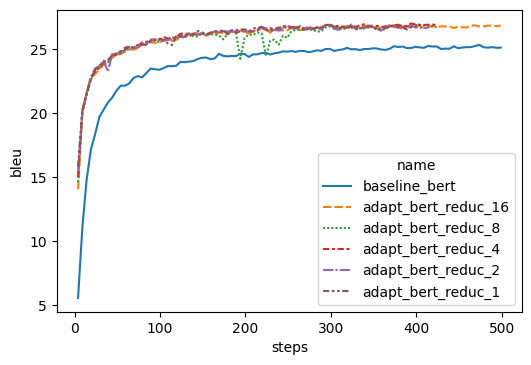
\includegraphics[width=0.95\textwidth]{img/adapter_bert_baseline_adapters.png}}
    \centering
    \caption{Comparison between baseline BERT model and adapters model with different ratio.}
    \label{img:adapt_bert_ratio}
\end{figure}

We can see from Figure \ref{img:adapt_bert_ratio} the comparison between different size of the ratio. The difference between the ratios are pretty minimal and it suggests that there is not much benefit in enlarging the adapters for the normal size BERT. It is possible that for large size model such as BERT, it is no longer trivial to just append adapters to fine-tune the model. As we recall from Section xxx, the biggest problem of using BERT is the difference in the output layers where we understand that BERT was trained using MLM objective. The MLM objective is naturally different from the normal machine translation objective such as autoregression.

\subsection{Position of adapters (encoder vs decoder)}
\subsubsection{Experiment setup}
We would like to see the importance of adapters when put in different place. Since in this work we are working with sequence-to-sequence architecture, we would like to see whether only incorporating adapters on one side can already beneficial and hence reducing the weights addition to the model.

\subsubsection{Experiment result}

\begin{figure}[h]
    {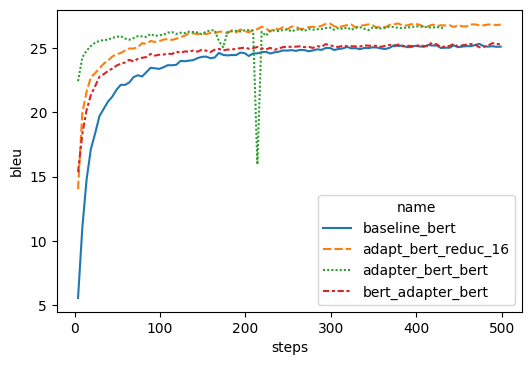
\includegraphics[width=0.95\textwidth]{img/bert_pos.png}}
    \centering
    \caption{Comparison between baseline BERT model and adapters model where the adapters are placed in three different setups: 1) Adapters in both encoder and decoder (\texttt{adapt\_bert\_reduc\_16}); 2) Adapters only in encoder (\texttt{adapter\_bert\_bert}); 3) Adapters only in decoder (\texttt{bert\_adapter\_bert}).}
    \label{img:adapt_bert_pos}
\end{figure}
We can see from Figure \ref{img:adapt_bert_pos} that by just adding the adapters on the encoder part, we already see an improvement and outperform the baseline model. If we remember from the previous chapter where we use the adapters on both side of encoder and decoder, we managed to get around 27. By adding the adapters on the encoder only, we can already see that the model eventually managed to achieve similar performance as if we add the adapters in both side. For the decoder, on the other hand, we can see that there is no benefit in adding the adapters as there are no improvement in terms of BLEU compared to the baseline.

It seems that by adding the adapters on the encoder and fine-tune it is more cost effective compared to the decoder. With this finding we can possibly reduce the cost of fine-tuning using adapters by half when we do not include the adapters on the decoder.

\subsection{Position of pre-training models (encoder vs decoder)}
\subsubsection{Experiment setup}
In this section, we would like to see the importance of having the pre-training models as the initial weights in either the encoder or decoder. In addition to that, we also expand the experiment further by trying to understand the correlation of adding adapters on top of the randomly set weights.

We start by defining the definition of the setup in this experiments. In the previous Chapter, we have already introduced randomly set experiment where we instantiate the base Transformer model with only random weights. We then fine-tune the base Transformer model by only updating the adapters and cross-attention layer. In this setup, we are doing experiments in similar concept except that we only initialized the random weights on either the encoder and decoder. We then perform similar setup as in the Chapter xxx (position of adapters) where we put the adapters only in the encoder or decoder.

The purpose of the experiments are:
\begin{itemize}
    \item We want to understand further the importance of the pre-training model when fine-tuned with adapters. By initializing the model with BERT only in one component, we can see whether it is necessary to use BERT on both components when adapters are incorporated.
    \item We want to understand the capability of adapters when either one of the components do not contain useful information (relative to BERT). We would like to see whether the adapters can recover or even outperform some of the performance that we have already gathered from the previous chapters and sections.
\end{itemize}

\subsubsection{Experiment results}
\paragraph{Randomly set weights on encoder}
In this section, we perform comparison amongst models that use adapters in both encoder and decoder, only in encoder, and only in decoder. We would like to see what is the impact of the randomly set weights encoder with the adapters. The main question that we would like to answer is "Compared to the BERT baseline, can adapters restore the missing gap when the encoder does not contain useful information (relative to BERT)?"

\begin{figure}[h]
    {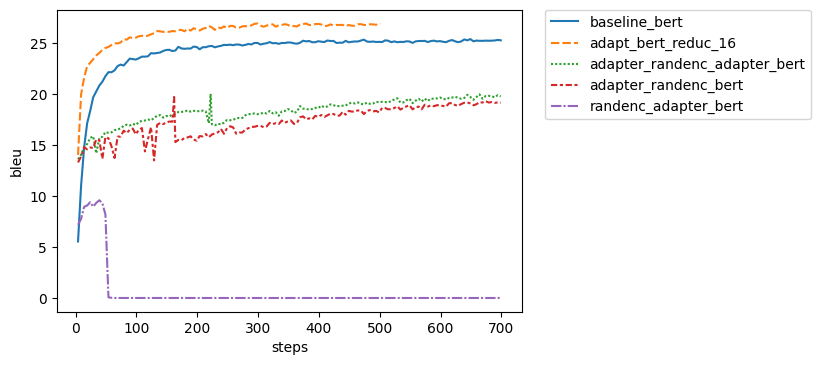
\includegraphics[width=0.95\textwidth]{img/adapter_bert_randenc.png}}
    \centering
    \caption{Comparison between baseline BERT model and adapters model where the adapters are placed in three different setups: 1) Adapters in both encoder and decoder (\texttt{adapt\_bert\_reduc\_16}); 2) Adapters only in encoder (\texttt{adapter\_bert\_bert}); 3) Adapters only in decoder (\texttt{bert\_adapter\_bert}) and the decoder is initialized with BERT while the encoder is initialized with random numbers.}
    \label{img:adapt_bert_randenc}
\end{figure}

We can see from Figure \ref{img:adapt_bert_randenc} that when adapters are appended in both components, we get to almost 20 in BLEU score. This is relatively higher than the other two setup. Compared to the baseline, we are missing 4 points in BLEU when we set the weights on encoder as completely random. This means that the encoder contains relatively important information for the adapters to restore.

Despite missing 4 points in BLEU, we would like to see the performance of the adapters when compared to the model that only fine-tuned on the cross-attention layer. We treat this model as the baseline for this section. We can see that the model that was only fine-tuning the cross-attention layer can not learn at all while the adapters can perform significantly better. This marks the capability of the adapter when faced with randomly set encoder.

When the adapters are removed from the decoder, we see a degradation in performance in about 1 BLEU. However, when the adapters are removed from the encoder, we can see the performance is completely depleted during the training. We also see the same behaviour on the next section when the weights on the decoder is set randomly. This tells us that there is some incompatibility on the weights (random and BERT) where it is not trivial to fine-tune the cross-attention layer without further adjustment on the base model's weights.

\paragraph{Randomly set weights on decoder}
Similar to Section xxx (**previous section**), we perform comparison amongst different setup in the adapters placement: adapters in both encoder and decoder, only in encoder, and only in decoder. We would like to understand the impact of the randomly set weights decoder while fine-txfuned with adapters. The main question in this experiment is "Compared to the BERT baseline, can adapters restore the missing gap when the decoder does not contain useful information (relative to BERT)?"

In contrast to when the randomly set weights is in encoder side, we can see from Figure \ref{img:adapt_bert_randdec}, the model have close performance to the one we have on BERT baseline. This tells us that the pre-training weights in encoder are more important than in decoder when we have adapters on both side. However, when remove the adapters on the encoder side, we see similar performance as in the previous section where the performance completely drop to 0 in the middle of training. This further our arguments that adapters are necessary to adjust the weights in the model so that the cross-attention layer can work properly.

\begin{figure}[h]
    {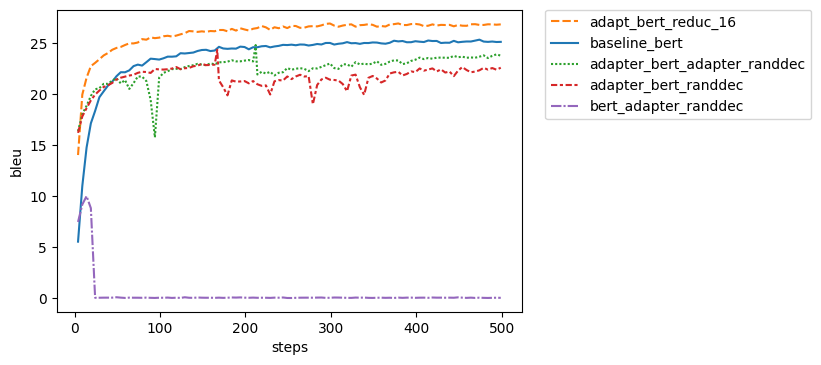
\includegraphics[width=0.95\textwidth]{img/adapter_bert_randdec.png}}
    \centering
    \caption{Comparison between baseline BERT model and adapters model where the adapters are placed in three different setups: 1) Adapters in both encoder and decoder (\texttt{adapt\_bert\_reduc\_16}); 2) Adapters only in encoder (\texttt{adapter\_bert\_bert}); 3) Adapters only in decoder (\texttt{bert\_adapter\_bert}) and the encoder is initialized with BERT while the decoder is initialized with random numbers.}
    \label{img:adapt_bert_randdec}
\end{figure}

On the other hand, when we remove the adapters from the decoder side, we can see that the performance is not as bad as when the adapters are removed from the encoder, but we still see a reduction in performance. We see around < 1 BLEU when the model reach 400k steps in the training stage.

\section{BERT size reduction}
\subsection{Zeroing columns}
\subsubsection{Experiment setup}
In this experiment, we will focus on soft reduction of BERT weights by zeroing the weights on every even index columns and rows in both Transformer body as well as in the embedding weights. The way we set this experiments by first manually editing the weights from BERT offline and then use the weights as the pre-trained models that later we will fine-tune using adapters. We further refer this setup as \texttt{zbert} for the rest of this writing.

Other than removing the columns, we also experimenting similar to Section xxx by initializing the adapters either on the encoder or the decoder. The goal of this particular experiments is to understand the behaviour of the model when the pre-trained models are replaced with this particular setup.

\subsubsection{Comparison with BERT baseline (full BERT fine-tuning)}
We first compare the model without adapter and only fine-tuning the cross-attention layers on \texttt{zbert} model. We use \texttt{zbert} weights on both encoder and decoder so that it is comparable to the BERT baseline.

\begin{figure}[h]
    {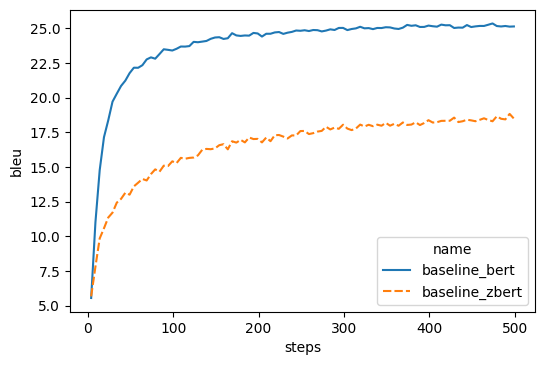
\includegraphics[width=0.95\textwidth]{img/baseline_zbert.png}}
    \centering
    \caption{Comparison between baseline BERT model and baseline \texttt{zbert} models.}
    \label{img:baseline_zbert}
\end{figure}

\begin{figure}[h]
    {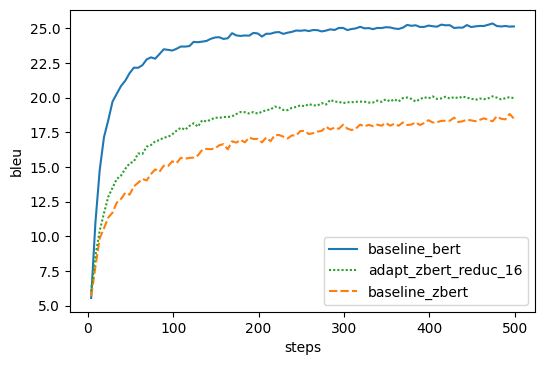
\includegraphics[width=0.95\textwidth]{img/adapter_zbert.png}}
    \centering
    \caption{Comparison between baseline BERT model, baseline \texttt{zbert} and adapters \texttt{zbert} models.}
    \label{img:adapter_zbert}
\end{figure}

We continue our experiment by fine-tuning \texttt{zbert} model that is instantiated on both encoder and decoder side with adapters. We can see in Figure \ref{img:baseline_zbert} that we are losing performance of about 4 BLEU. This is quite significant as this represents we are losing various important features from original BERT model. To see whether we can recover some of the performance with adapters, we perform a simple experiment where we include the adapters during the fine-tuning. We can see from the Figure \ref{img:adapter_zbert}, that we only manage to just recover 1 BLEU with reduction ratio of 16.

\begin{figure}[h]
    {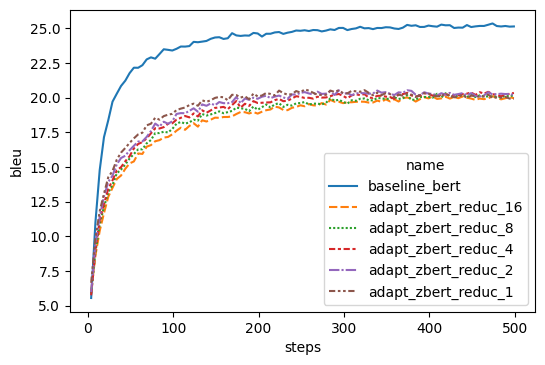
\includegraphics[width=0.95\textwidth]{img/adapter_zbert_ratio.png}}
    \centering
    \caption{Comparison between baseline BERT model and different reduction ratio of \texttt{zbert} models.}
    \label{img:adapter_zbert_ratio}
\end{figure}

From Figure \ref{img:adapter_zbert_ratio}, when we increase the size of the reduction ratio, initially we can see some improvement compared the higher ration. However, when they eventually converge to the similar performance by the end of training. From this we can understand that there is still a limitation for adapters to achieve certain performance, depending on the base pre-trained model that choose to use.

\subsubsection{Adapters position}
In this section, we are trying to understand whether the position of both adapters and the pre-training models affect the model performance similar as we have seen in Section xxx. We use similar setup as in the previous Section with exception that we use \texttt{zbert} as the pre-trained model instead of the original BERT model.

\begin{figure}[h]
    {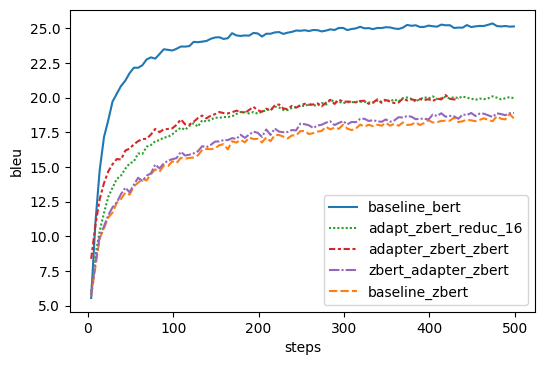
\includegraphics[width=0.95\textwidth]{img/zbert_pos.png}}
    \centering
    \caption{Comparison between baseline BERT model, baseline \texttt{zbert} model, adapters in both encoder and decoder of \texttt{zbert} model (\texttt{adapt\_zbert\_reduc\_16}), adapters only in encoder of \texttt{zbert} model (\texttt{adapter\_zbert\_zbert}), and adapters only in decoder of \texttt{zbert} model (\texttt{zbert\_adapter\_zbert}).}
    \label{img:zbert_pos}
\end{figure}

We can see from Figure \ref{img:zbert_pos} that when we include adapters on both encoder and decoder, we can outperform the baseline \texttt{zbert} in around 2 BLEU points. This shows that similar to the models that use BERT as the pre-training models, the adapters can help to improve the performance further even though some of the information already missing in the base model.

Furthermore, we can also see that similar to the BERT model that was fine-tuned with adapters, using adapters only on the encoder side performs much better than in the decoder side. Other than that, we can also see that incorporating adapters only on the encoder side helps the model to achieve better performance faster compared to the model that uses adapters on both side. This further support our hypothesis that updating the representation on the encoder side is more beneficial. If we take a look deeper on model with adapters on the decoder side, the performance is close to the baseline model where we only fine-tune the cross-attention layer. This could mean that fine-tuning the decoder only may not be enough to achieve better performance when the representation from the source side is constant.

\subsection{Model downscaling}
\subsubsection{Experiment setup}
This experiment is the continuation from \texttt{zbert} where we zeroing out some of the matrix elements. Specifically, instead of just zeroing out the elements, we now completely removing those elements from the matrix. The way we do this is similar to the one we do on \texttt{zsbert}. We remove the matrix elements on every even columns and rows in both Transformer body as well as the embedding weights. We similarly do the weights processing offline before using it as the pre-training base model. For the rest of this writing, we refer to this setup as \texttt{zsbert}.

Furthermore, we also follow similar setup as in Section xxx where we experiment on the position of the adapters position. The goal of this experiments is that we would like to understand the behaviour of the model compared to the baseline as well as \texttt{zbert}.

\subsubsection{Comparison with BERT baseline and zbert}

\begin{figure}[h]
    {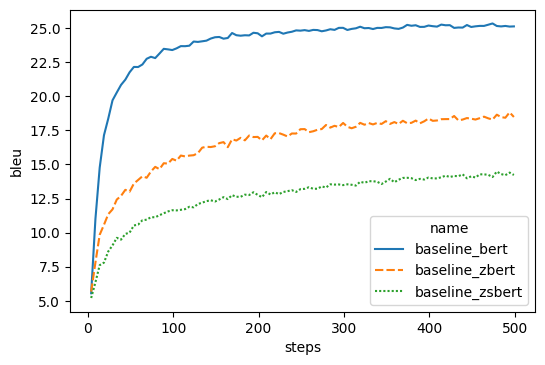
\includegraphics[width=0.95\textwidth]{img/baseline_zsbert.png}}
    \centering
    \caption{Comparison between baseline BERT model and baseline \texttt{zsbert} model.}
    \label{img:baseline_zsbert}
\end{figure}

\begin{figure}[h]
    {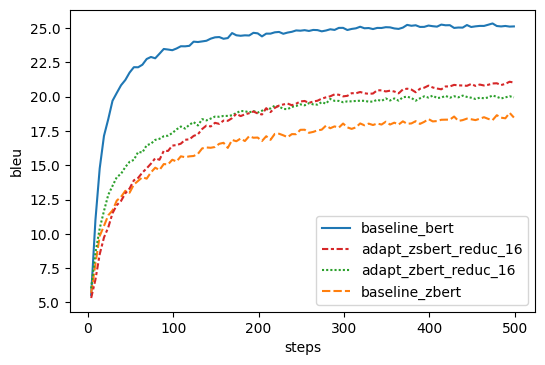
\includegraphics[width=0.95\textwidth]{img/adapter_zsbert.png}}
    \centering
    \caption{Comparison between baseline BERT model, baseline \texttt{zsbert} and adapters \texttt{zsbert} models.}
    \label{img:adapter_zsbert}
\end{figure}

We begin with the comparison of \texttt{zsbert} with the BERT baseline. We can see from Figure \ref{img:baseline_zsbert} that the performance degrades significantly for almost 10 BLEU. This is also significantly worse than \texttt{zbert} where we only lose 5 BLEU. After some investigation, we realize that it is not straightforward to remove weights from the network as the computation of layer normalization layer in the Transformer will compute different results as the normalization scaling factor will also be different. With manual evaluation, we found that there is a small different between weights that only zeroed and weights that is completely removed. Despite the small difference in the output of layer normalization, the error will be propagated to the top layers and causing the result to differ significantly.

From the aforementioned challenge, we also interested to see whether adapters have the capability to mitigate the problem and able to recover some of the performance. We can see from Figure \ref{img:adapter_zsbert} that adapters with 16 ratio already managed to improve the performance up to 6 BLEU. This shows another capability of adapters to intermediate numerical errors in the middle of the layers.

\begin{figure}[h]
    {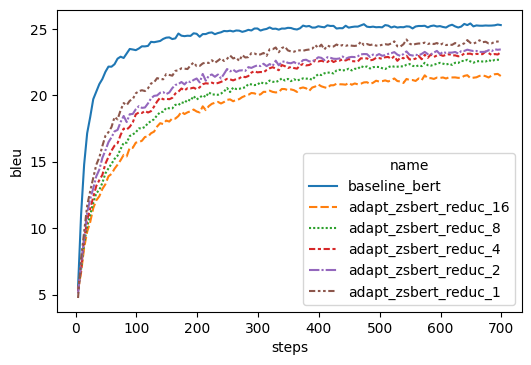
\includegraphics[width=0.95\textwidth]{img/adapter_zsbert_ratio.png}}
    \centering
    \caption{Comparison between baseline BERT model and different reduction ratio of \texttt{zsbert} models.}
    \label{img:adapter_zsbert_ratio}
\end{figure}

In Figure \ref{img:adapter_zsbert_ratio}, when the adapters reduction ratio is further reduced, we can see that the performance also improving up to the point where it has close performance to the baseline model. This remarks a prominent result as we can see from Table \ref{tab:numvars} that the total number of weights (including adapters) is reduced significantly.

\begin{table}[]
    \centering
    \begin{tabular}{@{}cccc@{}}
        \toprule
        \textbf{Name}                                                               &
        \textbf{\begin{tabular}[c]{@{}c@{}}\# Trainable\\ Variables\end{tabular}}   &
        \textbf{\begin{tabular}[c]{@{}c@{}}\# Untrainable\\ Variables\end{tabular}} &
        \textbf{\begin{tabular}[c]{@{}c@{}}\# Total\\ Variables\end{tabular}}                                                \\ \midrule
        \textbf{Adapters ratio 16}                                                  & 7.736.826  & 95.143.296  & 102.880.122 \\
        \textbf{Adapters ratio 8}                                                   & 8.179.770  & 95.143.296  & 103.323.066 \\
        \textbf{Adapters ratio 4}                                                   & 9.065.658  & 95.143.296  & 104.208.954 \\
        \textbf{Adapters ratio 2}                                                   & 10.837.434 & 95.143.296  & 105.980.730 \\
        \textbf{Adapters ratio 1}                                                   & 14.380.986 & 95.143.296  & 109.524.282 \\
        \textbf{Normal BERT}                                                        & 28.990.078 & 218.819.328 & 247.809.406 \\ \bottomrule
    \end{tabular}
    \caption{Total trainable variables in \texttt{zsbert} with adapters on different ratio vs normal BERT model}
    \label{tab:numvars}
\end{table}

\subsubsection{Adapters position}

\begin{figure}[h]
    {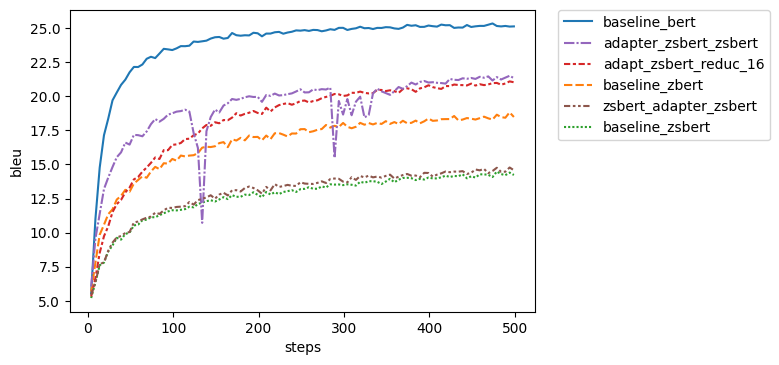
\includegraphics[width=0.95\textwidth]{img/zsbert_pos.png}}
    \centering
    \caption{Comparison between baseline BERT model, baseline \texttt{zsbert} model, adapters in both encoder and decoder of \texttt{zsbert} model (\texttt{adapt\_zsbert\_reduc\_16}), adapters only in encoder of \texttt{zsbert} model (\texttt{adapter\_zsbert\_zsbert}), and adapters only in decoder of \texttt{zsbert} model (\texttt{zsbert\_adapter\_zsbert}).}
    \label{img:zsbert_pos}
\end{figure}

From Figure \ref{img:zsbert_pos}, similar to the \texttt{zbert} experiments, we can see similar behaviour as models that are fine-tuned with adapters outperform the baseline \texttt{zsbert} and \texttt{zbert} models. Compared to \texttt{zbert} experiments, we notice a bigger gap in performance improvement in \texttt{zsbert}. In \texttt{zbert}, the difference between baseline and adapters is in the range of 5 BLEU. On the other hand, in \texttt{zsbert} we see the improvement is in the range of 8 BLEU. This result is particularly interesting for us as we recall from the baseline experiments that due to the numerical error from the layer normalization, we expect the difference is similar to \texttt{zbert} and have lower performance than we currently have. To further deep-dive on this, we refer to Figure \ref{img:zbert_vs_zsbert} to show the comparison between adapters in \texttt{zbert} and \texttt{zsbert}. We compare the adapters model with equal reduction ratio (16) between these two setup. We can see that initially \texttt{zsbert} performs worse than \texttt{zbert}. After some steps, we can see the performance in \texttt{zbert} starting to stall but not in \texttt{zsbert}. We hypothesize this relates to similar reason that we state on the original BERT model where we could not see any improvement when we increase the reduction ratio. \texttt{zsbert} is half the size of original BERT model and \texttt{zbert} model, it is probably that reducing the weights and essentially modifying the architecture by incorporating adapters help the model to achieve better performance.

\begin{figure}[h]
    {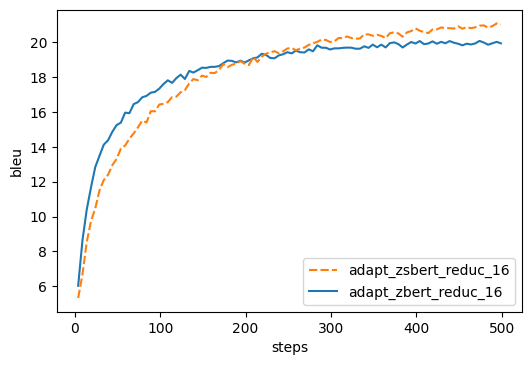
\includegraphics[width=0.95\textwidth]{img/zbert_vs_zsbert.png}}
    \centering
    \caption{Comparison adapters performance in \texttt{zsbert} and \texttt{zbert}. Both are using reduction ratio 16 and the adapters are placed on encoder and decoder.}
    \label{img:zbert_vs_zsbert}
\end{figure}

We see similar behaviour as we see on \texttt{zbert} experiments in regards of the position of the adapters. In Figure \ref{img:zsbert_pos}, the benefit of incorporating adapters on the encoder side is also apparent and outperform the decoder counterpart. We can also see a similar behaviour where eventually the performance of model with adapters on encoder outperform model with adapters on both side. Furthermore, we also see similar behaviour as in \texttt{zbert} for models with adapters where the performance is very close to the baseline and not improving as much as the encoder side. We hypothesize the same reason as we have stated in \texttt{zbert} could apply in \texttt{zbert} as well. Essentially, we need to modify the representation on the encoder side in order to achieve better performance.
